\documentclass{standalone}
\usepackage{tikz}

\begin{document}

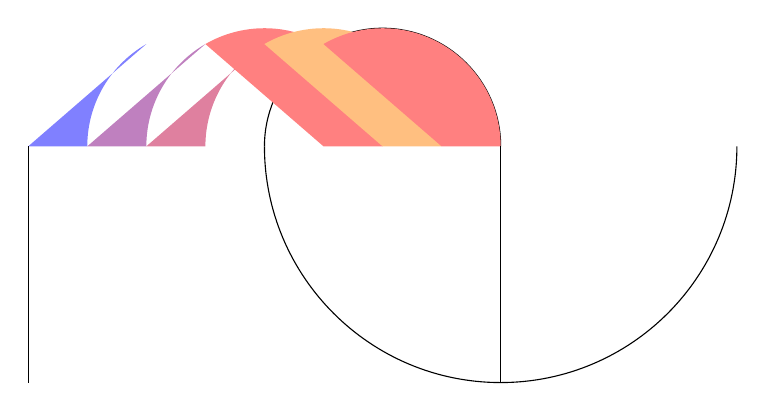
\begin{tikzpicture}[scale=1.5]
    % Draw the outer arc
    \draw (0,0) arc (180:360:2);
    
    % Draw the inner arc
    \draw (0,0) arc (180:0:1);
    
    % Fill the segments with different colors
    \fill[blue!50] (-2,0) -- (-1.5,0) arc (180:120:1) -- cycle;
    \fill[violet!50] (-1.5,0) -- (-1,0) arc (180:120:1) -- cycle;
    \fill[purple!50] (-1,0) -- (-0.5,0) arc (180:120:1) -- cycle;
    \fill[red!50] (0.5,0) -- (1,0) arc (0:120:1) -- cycle;
    \fill[orange!50] (1,0) -- (1.5,0) arc (0:120:1) -- cycle;
    \fill[red!50] (1.5,0) -- (2,0) arc (0:120:1) -- cycle;
    
    % Draw the vertical lines
    \draw (-2,0) -- (-2,-2);
    \draw (2,0) -- (2,-2);
\end{tikzpicture}

\end{document}